\documentclass[12pt]{article}

\usepackage{sbc-template}
\usepackage{graphicx,url}
\usepackage[utf8]{inputenc}
\usepackage[brazil]{babel}

     
\sloppy

\title{Ranking de agrupamento de Células em imagens de exames de Papanicolau}

\author{Francisco Gleidson Nascimento de Queiroz\inst{1} Daniel Silva Ferreira\inst{2} }


\address{Departamento de Computação\\Instituto Federal de Educação, Ciência e Tecnologia do Ceará(IFCE)\\
 Maracanaú -- CE -- Brasil
}

\begin{document} 

\maketitle

\begin{abstract}
  There are several challenges related to the segmentation of cervical cell images. This article seeks to estimate the density of a group of cells, considering that specialists tend to observe cell fields with less overlaps, seeking a better approach for segmentation and detection of nuclei in images of exams with these cells.
\end{abstract}
     
\begin{resumo} 
  Existem diversos desafios relacionados a segmentação de imagens de células cervicais. Este artigo busca estimar a densidade de um grupo de células, considerando que especialistas tendem a observar campos celulares com menos sobreposições, buscando uma melhor abordagem para a segmentação e detecção de núcleos em imagens de exames com estas células.
\end{resumo}


\section{Introdução}

A quantificação das propriedades de células cervicais tem sido utilizada na detecção de lesões pré-cancerígenas do colo do útero. A abordagem tradicional se baseia na busca visual em lâminas do exame Papanicolau, o objetivo é encontrar padrões que sejam correlacionados com células anormais. O maior desafio nesse caso é a inspeção manual, uma tarefa que não atenderá a demanda de acordo com o crescimento da população \cite{silva2018detecccao}.

Um dos tipos mais comuns de câncer entre as mulheres é o  câncer cervical, com cerca de 527.000 novos casos a cada ano  em todo o mundo, e quase 80\% desse casos ocorrem em países com baixa renda. Este câncer foi responsável pela morte de265.000 mulheres em 2012, e 87\% dessas mortes ocorreramem países em desenvolvimento \cite{ramalho2015cell}. O núcleo possui várias informações para detecção de anomalias sendo de fundamental importância sua análise e assim o desenvolvimento de ferramentas computacionais  afim de que a análise possa ser consistente reduzindo principalmentede resultados falsos negativos.

Trabalhos recentes têm mostrado que algoritmos de segmentação funcionam de forma diferente dependendo do nível de sobreposição celular da imagem processada. Então identificar a densidade dos agrupamentos de células cervicais e criar um ranking das densidades pode ajudar na identificação do nível de sobreposição celular destes agrupamentos.

Para tentar estimar a densidade de um grupo de células inicialmente iremos estimar a densidade de células cervicas em um agrupamento utilizando a distância entre núcleos, pois a segmentação em agrupamentos densos é complexa.

\section{Fundamentação Teórica} \label{sec:firstpage}

O autor propôs uma segmentação automática utilizando o método de múltiplas células cervicais sobrepostas em microimagens
escópicas com partição de superpixel e célula refinamento de contorno. Primeiramente para determinar a área de busca, 
as massas celulares são detectadas através da geração de superpixel e \textit{adaptive triangle thresholding}. Para definir
a posição da célula, núcleos das células são extraídas por limite local baseado em janela – remoção
e remoção de valores discrepantes. Finalmente, para delimitar o limite áreas das células sobrepostas, o citoplasma da célula é segmentado e particionado por superpixel e refinamento de contorno em nível celular. Experimentos mostraram
que o método apresentou resultados competitivos em dois conjuntos de dados de desafio público, com
pareados aos métodos mais modernos. A principal contribuição é o particionamento de superpixel e no refinamento de contorno em
segmentação do citoplasma celular, o que aumenta a precisão de sobreposição de limites de células para o nível de última geração por
desempenho \cite{lee2016segmentation}.

O autor se concentrou na extração de limites individuais do citoplasma e dos núcleos de sobreposição cervical em
imagens citológicas adquiridas em diferentes planos focais (\textbf{FOV}). O método difere de outras abordagens, pois processa não apenas a profundidade extensa de representação de imagem de campo (\textbf{EDF}), mas também nas imagens \textbf{FOV} para encontrar as bordas de citoplasmas sobrepostos. Foram combinados algoritmos interligados para fornecer um eficiente \textit{pipeline} para núcleo automatizado e segmentação de citoplasma: superpixel combinado com diagramas de \textbf{Voronoi} ou \textbf{SPVD}, seguido por algoritmos usando cálculo de variações para construir mapas de borda, processados usando métodos morfológicos matemáticos, reconstrução aliada à elipse detectoras e, finalmente, fornecer um limite de citoplasma refinado As avaliações dos conjuntos de dados mostram desempenhos qualitativos e quantitativos, usando um programa de computador completamente automatizado. O desempenho quantitativo apresenta Coeficiente de Dados médio superior a 87\% \cite{ramalho2015cell}.

O autor apresentou ferramentas para classificação de células e recuperação de imagens, incluindo o descritor de atributos radiais (\textit{Radial Feature Descriptor} - \textbf{RFD}) para categorizar padrões normais e anormais de células cervicais. O \textbf{RFD} define retas igualmente espaçadas ao redor do núcleo que são responsáveis por capturar variações de intensidade na membrana citoplasmática. Ele combina os atributos de intensidade com atributos de textura provenientes do cálculo da distribuição de cromatina no núcleo sem a necessidade de segmentação do citoplasma. Para avaliar os resultados foram utilizadas duas bases de imagens: \textbf{Herlev}, uma base pública; e \textbf{CRIC} uma base de imagens apresentadas na tese. As células individuais da base \textbf{CRIC} foram obtidas pelo uso de um algoritmo de segmentação de núcleos proposto. Foi realizado experimentos de classificação de imagens e de recuperação de imagens baseada em conteúdo (\textit{Content-Based Image Retrieval} - \textbf{CBIR}). As células com o algoritmo \textit{Random Forest} foram classificadas utilizando a metodologia bootstrap para criar os conjuntos de treinamento e teste. Os experimentos \textbf{CBIR} foram realizados utilizando a distância cosseno como métrica de similaridade. As principais contribuições foram: um novo método para segmentação de núcleos de células cervicais; \textbf{RFD}, um extrator de atributos de células cervicais; \textbf{pyCBIR}, uma nova ferramenta para recuperação de imagens. Os experimentos de classificação foram mensurados em termos do índice \textit{Kappa} (\textbf{k}) e da taxa de falso negativos (\textit{False Negative Rate} - \textbf{FNR}), foi calculado o \textit{Mean Average Precision} (\textbf{MAP}) para avaliar os experimentos CBIR \cite{silva2018detecccao}.

O autor buscou verificar uma melhor abordagem para a detecção precoce de câncer na análise de imagens provenientes de lâminas de cavidade oral coradas com Papanicolau. Ele comparou os métodos de \textit{Deep Learning} para segmentação e detecção de objetos para localização de núcleos em imagens provenientes de lâminas de três diferentes pacientes. O melhor resultado indica um \textbf{IoU} de 0,59 para a segmentação e 0,81 para a detecção de objetos. Os resultados mostraram que a detecção de objetos usando o modelo \textit{Faster R}-\textbf{CNN} possui potencial de ser usado juntamente com um modelo de classificação de imagens para auxiliar na detecção precoce de câncer \cite{matias2021localizaccao}.

O autor propõe um método baseado em Redes Neurais Convolucionais para detectar automaticamente os núcleos de células cervicais. Após ser realizado o treinamento com um conjunto de dados disponibilizados pelo \textit{Overlapping Cervical Cytology Image Segmentation Challenge} - \textbf{ISBI 2014}, suas camadas completamente conectadas são convertidas em camadas convolucionais para permitir o processamento de imagens de qualquer tamanho. Os resultados obtidos foram comparados com os de outros participantes do \textbf{ISBI 2014} e também com trabalhos que utilizaram o mesmo conjunto de dados. Os resultados experimentais indicaram que a metodologia proposta provê uma detecção de núcleos com métricas de precisão e \textit{recall} comparáveis com os métodos do estado da arte em detecção de núcleos de células cervicais. Em casos que o tempo de processamento não seja um limitador, utilizando técnicas de morfologia matemática é possível melhorar ainda mais os resultados \cite{braz2018detecccao}.


\section{Metodologia}

Iremos definir alguns passos, no primeiro passo vamos detectar os agrupamentos celulares, no segundo passo detectar a quantidade de núcleos em cada grupo, no terceiro passo calcular métrica de distância entre os núcleos e por fim comparar o ranking obtido com o ranking computado a partir do GT.

\section{Conclusões}

Section titles must be in boldface, 13pt, flush left. There should be an extra
12 pt of space before each title. Section numbering is optional. The first
paragraph of each section should not be indented, while the first lines of
subsequent paragraphs should be indented by 1.27 cm.

\subsection{Subsections}

The subsection titles must be in boldface, 12pt, flush left.



Figure and table captions should be centered if less than one line
(Figure~\ref{fig:exampleFig1}), otherwise justified and indented by 0.8cm on
both margins, as shown in Figure~\ref{fig:exampleFig2}. The caption font must
be Helvetica, 10 point, boldface, with 6 points of space before and after each
caption.

\begin{figure}[ht]
\centering
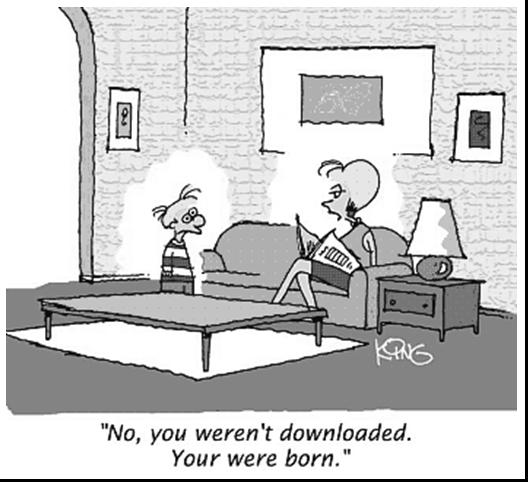
\includegraphics[width=.5\textwidth]{fig1.jpg}
\caption{A typical figure}
\label{fig:exampleFig1}
\end{figure}

\begin{figure}[ht]
\centering
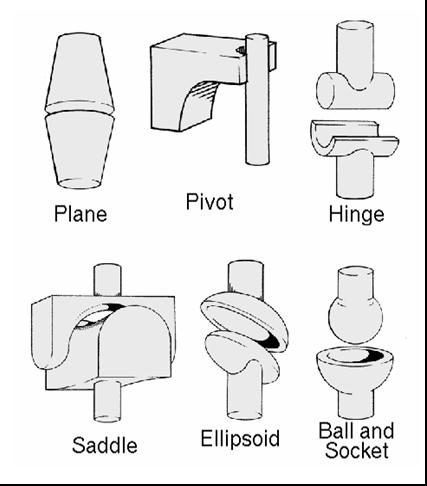
\includegraphics[width=.3\textwidth]{fig2.jpg}
\caption{This figure is an example of a figure caption taking more than one
  line and justified considering margins mentioned in Section~\ref{sec:figs}.}
\label{fig:exampleFig2}
\end{figure}

In tables, try to avoid the use of colored or shaded backgrounds, and avoid
thick, doubled, or unnecessary framing lines. When reporting empirical data,
do not use more decimal digits than warranted by their precision and
reproducibility. Table caption must be placed before the table (see Table 1)
and the font used must also be Helvetica, 10 point, boldface, with 6 points of
space before and after each caption.

\begin{table}[ht]
\centering
\caption{Variables to be considered on the evaluation of interaction
  techniques}
\label{tab:exTable1}
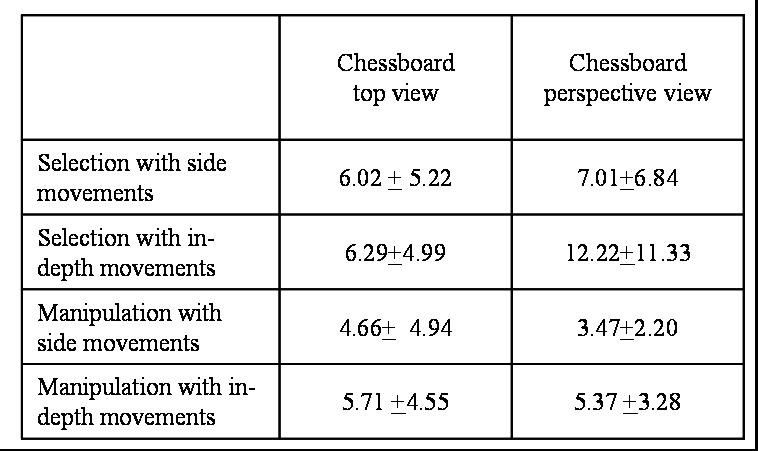
\includegraphics[width=.7\textwidth]{table.jpg}
\end{table}

All images and illustrations should be in black-and-white, or gray tones,
excepting for the papers that will be electronically available (on CD-ROMs,
internet, etc.). The image resolution on paper should be about 600 dpi for
black-and-white images, and 150-300 dpi for grayscale images.  Do not include
images with excessive resolution, as they may take hours to print, without any
visible difference in the result. 

\section{Referências Bibliográficas}

Bibliographic references must be unambiguous and uniform.  We recommend giving
the author names references in brackets, e.g. \cite{knuth:84},
\cite{boulic:91}, and \cite{smith:99}.

The references must be listed using 12 point font size, with 6 points of space
before each reference. The first line of each reference should not be
indented, while the subsequent should be indented by 0.5 cm.

\bibliographystyle{sbc}

\bibliography{sbc-template}

\end{document}
